\chapter{L'oscillateur contrôlé en tension (VCO)}
\label{chap:vco}
Le VCO est la partie qui s'occupe de générer un signal périodique à partir d'une tension continue. 
La fréquence du signal généré dépend de manière linéaire à la tension d'entrée avec comme relation
tension-fréquence : \unit{1}{\milli\volt} correspond à \unit{1}{\hertz}. Le comportement
souhaité du VCO est représente sur la figure \ref{fig:in-out-vco}.

\begin{figure}[ht]
	\centering
	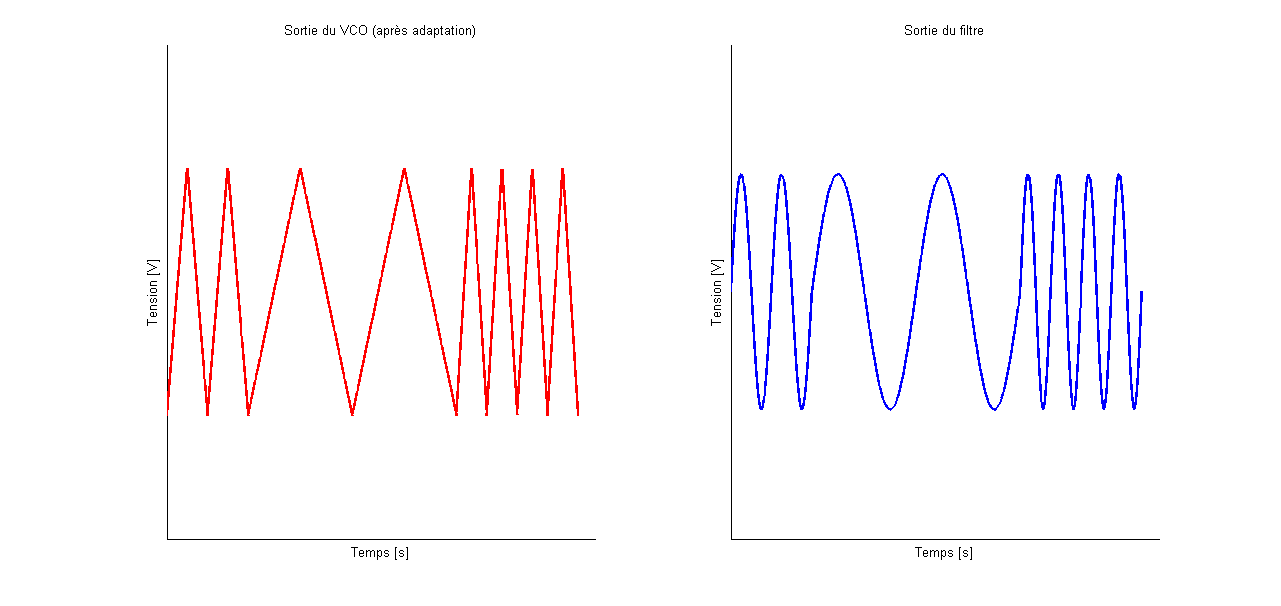
\includegraphics[scale=0.3]{img-vco/in-out.png}
	\caption{Relation entrée-sortie souhaitée du VCO.}
	\label{fig:in-out-vco}
\end{figure}

\section{Fonctionnement et théorie}
La figure \ref{fig:schema_bloc_vco} montre le schéma-bloc du VCO.

\begin{figure}[ht]
	\centering
	\includegraphics[scale=0.3]{img-vco/schema_bloc_vco.png}
	\caption{Schéma bloc du VCO.}
	\label{fig:schema_bloc_vco}
\end{figure}

Le VCO est composé des 3 blocs suivants :
\begin{itemize}
	\item le contrôleur de l'intégrateur qui se compose lui-même d'un switch et d'un sommateur.
	\item l'intégrateur.
	\item le trigger de Schmitt (bascule à hystérèse).
\end{itemize}

Le signal d'entrée $in$ est constant et vaut $\alpha$. Soient $V_L$ la
tension de basculement inférieure du trigger, $V_H$ la tension de 
basculement supérieure et $V_{CC}$ la tension d'alimentation du trigger.
Si la sortie du trigger de Schmitt (\textit{contrôle} sur la figure \ref{fig:schema_bloc_vco}) 
vaut $0$, la sortie du switch vaut $0$. Dès lors, la sortie du bloc contrôleur de l'intégrateur vaut $-\alpha$. Après passage dans l'intégrateur, nous avons la 
droite $-K\alpha t$ avec $K$ la constante de temps de l'intégrateur. La sortie du trigger
restera à $0$ tant que la sortie de l'intégrateur est supérieure à $V_L$. Lorsque la sortie
de l'intégrateur atteint $V_L$, le trigger bascule et sa tension de sortie devient $V_{CC}$. 
Le switch change d'état et sa sortie devient $\alpha$. La sortie dû contrôleur de l'intégrateur
devient donc $\alpha$. Après passage dans l'intégrateur, $\alpha$ devient $K\alpha t$. 
La sortie du trigger restera à $V_{CC}$ tant que la sortie de l'intégrateur est inférieure à $V_H$.
Lorsque la sortie de l'intégrateur atteint $V_H$, le trigger bascule et sa tension de sortie devient
$0$. Le switch change à nouveau d'état, sa sortie devient $0$ et le cycle recommence.

La fréquence générée par le VCO pour une tension d'entrée $\alpha$ s'exprime 
en fonction de $K$ et de $\Delta V = \vert V_H - V_L\vert $ par la relation 
\[ f = \frac{K\alpha}{2\Delta V}. \]
L'amplitude du signal généré par le VCO est compris entre $V_H$ et $V_L$.


\section{Dimensionnement et circuit réel}
\paragraph{Circuit réel}
Sur la figure \ref{fig:circuit_vco} se trouve l'implémentation électronique du VCO décrit ci-dessus.

\begin{figure}[ht]
	\centering
	\includegraphics[scale=0.3]{img-vco/vco_circuit}
	\caption{Circuit du VCO}
	\label{fig:circuit_vco}
\end{figure}

\paragraph{Dimensionnement du trigger de Schmitt}
Le choix de placer le seuil supérieur $V_H$ à \unit{0}{\volt} 
et le seuil inférieur $V_L$ à \unit{-1}{\volt} est arbitraire. 
Cependant, la différence entre $V_H$ et $V_L$ doit rester au-dessus
de \unit{500}{\milli\volt} pour éviter une influence des tensions parasites.
% FIX : pas vraiment justifable, 500mV >> quelques mV des tensions parasites.
% On pourrait sans doute encore descendre plus bas.
Dans ce circuit, un trigger asymétrique est utilisé. Dès lors, le rapport
des résistances à utiliser se déduit des formules suivantes : 
\[ V_H = V_{REF}\left(1+\frac{R_2}{R_6}\right) \text{ et } V_L = V_{REF} + \frac{R_2}{R_6}\left(V_{REF}-V_{CC}\right). \]
Dans le montage du trigger asymétrique utilisé, $V_{REF}$, la tension à l'entrée
inverseuse du comparateur vaut \unit{0}{\volt}. Dès lors, $\frac{R_2}{R_6}=\frac{1}{15}$
avec la condition que $R_6 >> R_9$. Les valeurs de résistances choisies sont :

\begin{itemize}
	\item \unit{10}{\kilo\ohm} pour $R_2$ .
	\item \unit{150}{\kilo\ohm} pour $R_6$.
\end{itemize}

\paragraph{Dimensionnement de l'intégrateur}
Calculons maintenant la constante ($K$) du bloc intégrateur. 
Comme le signal de sortie est un signal triangulaire, le temps de montée et de descente est 
identique. Le temps de montée vaut donc $\frac{1}{2\cdot1} = \unit{0.5}{\second}$. 
La pente de montée de la droite est de \unit{1}{\milli\volt}/\unit{}{\second}. 
Le temps pour monter ou descendre de \unit{1}{\volt} est de \unit{1000}{\second}. 
Comme il doit valoir \unit{0.5}{\second}, la constante d'intégration vaut 2000. D'où 
$K=\frac{1}{R_1C_1} = 2000$ avec $C_1= \unit{100}{\nano\farad}$, $R_1 = \unit{5}{\kilo\ohm}$.
\paragraph{Dimensionnement du contrôleur de l'intégrateur}
Le contrôleur de l'intégrateur est constitué d'un amplificateur opérationnel 
en mode différentiel et d'un switch. L'équation constitutive de ce bloc est : 
$V_{IC}=2*V_+ - V_-$ avec $V_+$ la tension à l'entrée non-inverseuse et $V_-$
la tension à l'entrée inverseuse. La formule suivante permettant de déterminer
une relation entre les résistances est obtenue en appliquant KCL : 
\[ V_{IC}=V_+ \left(\frac{R_4 + R_5}{R_5}\right)-V_-\left(\frac{R_4}{R_5}\right). \] 
Cela donne donc $R_5 = R_4$. En prenant $R_5 =$ \unit{1}{\kilo\ohm}, $R_4$ vaut \unit{1}{\kilo\ohm}
et $R_3$ vaut \unit{10}{\kilo\ohm}.

\section{Confrontation  des mesures et de la théorie}
La figure \ref{fig:theory_vs_mesure} montre que la réalité est la théorie sont très proche.
Les différences observées sont dues à des imprécisions des valeurs des résistances et des 
capacités. Cela provient aussi du switch qui contrairement au modèle utilisé dans les 
simulations et les calculs possède une légère courbe d'hystérèse.
\begin{figure}[ht]
	\centering
	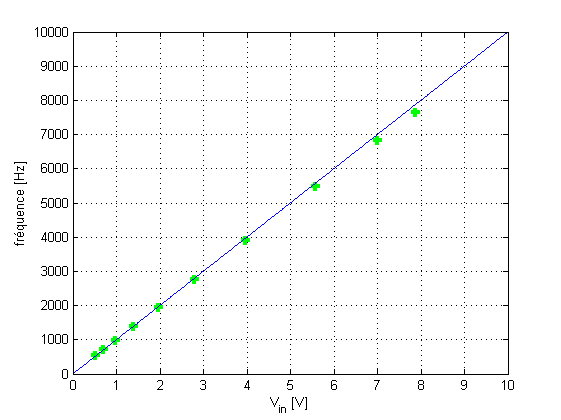
\includegraphics[scale=0.45]{img-vco/vco_vs_reality.png}
	\caption{Confrontations des théories et des mesures.}
	\label{fig:theory_vs_mesure}
\end{figure}